\section{Kernel Generation and Selection}
\label{sec:search}
Generation and selection turn the legal organizations into reusable plans.
Figure~\ref{fig:framework} follows Figure~\ref{fig:overview}'s inputs to
residency, layouts, concurrency, and handoffs.
The complete device path defines warm execution; preparation, including
compilation, is excluded.

\begin{figure}[t]
\centering
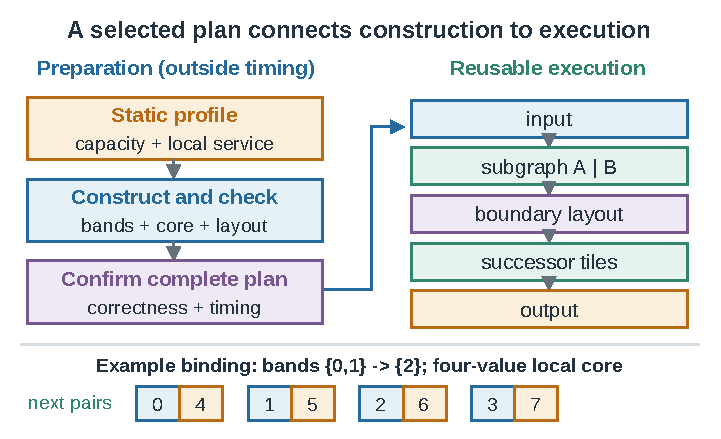
\includegraphics[width=\columnwidth]{figures/drawio/exports/system_architecture.pdf}
\caption{Preparation constructs and checks subgraph plans, then the selected
plan controls local execution and boundary exchange.}
\label{fig:framework}
\end{figure}

\noindent\textbf{Compatible realizations.}
Generation combines bands, regions, cores, storage, layouts, and bulk/pipelined
schedules while preserving arithmetic, precision, direction, normalization,
order, shape, and placement. Adaptation
costs remain included; missing compatible lowering remains a gap. Static
checks enforce dependencies and capacity; compilation exposes local allocation,
intermediate and temporary storage, and launch requirements. Numerical checks precede timing.
Failed checks remain recorded but untimed. Cache reuse requires matching
semantic, workload, hardware, and compilation assumptions.

\noindent\textbf{Service estimates.}
Services are keyed by arithmetic, core, tile shape, layout, and resource regime,
separating full and remainder tiles when necessary. Piecewise linear
interpolation stays within compatible measured regimes; missing coverage
requires measurement or an explicit gap. Composition respects predecessors,
buffers, and shared-resource contention: shared execution and memory capacity
can lengthen concurrent service intervals. Submission costs are added only when
absent from measured services. Estimates guide preparation; search instantiates
the resource characterization rather than constituting a contribution.

\noindent\textbf{Bounded selection and confirmation.}
Finite-budget selection uses bounded enumeration or model-guided exploration;
explicit evolutionary tuning adds multistart neighborhood mutation.
Multidimensional selection measures whole candidates before refining axes.
Compatible caches and calibration avoid repeated preparation. All modes share
semantic/resource constraints and retain complete organization costs.
Complete-plan timing confirms selection, separately from static ranking.
Organization comparisons distinguish explicit interventions from searched plans,
retaining actual mappings, tuning conditions, and confirmation protocols.
Finite search does not establish global optimality.
